\documentclass{report}
\usepackage[utf8]{inputenc}
\usepackage[T1]{fontenc}
\usepackage{graphicx}
\usepackage[croatian]{babel}
\graphicspath{{slike/}}
\usepackage{url}


\begin{document}
\title{Gaming računalo}
\author{Nera Borbelj}
\date{25.1.2024.}
\maketitle
\tableofcontents
\listoffigures

\chapter{Cijena i uporaba računala}
Računalo je namijenjeno za višestruku uporabu što uključuje 3D modeliranje, foto i video obradu, programiranje i igranje igrica. Jako je tiho i dovoljno jako za sve moje potrebe. Ukupna cijena ovog računala je otprilike 2.800€.
 
\chapter{Procesor}
AMD Ryzen 9 5950X 3.4 GHz, 16 jezgri.
\\ Odabrala sam ovaj procesor zbog osobnih potreba koje zahtjevaju brz i jak procesor, te taj isti obavlja to bez ikakvih problema.
\\Cijena: 364,99€
\\Izvor:  \url{https://www.amazon.com/dp/B0815Y8J9N?tag=pcpapi-20&linkCode=ogi&th=1&psc=1}
\begin{figure}[h]
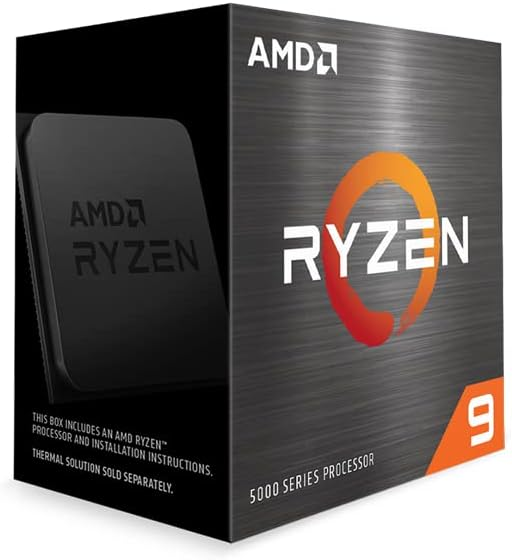
\includegraphics[width=8cm]{slike/procesor.jpg}
\caption{AMD Ryzen 9 5950X}
\end{figure}


\chapter{Grafička kartica}
Asus ROG STRIX GAMING OC GeForce RTX 3080 12GB
\\ Grafička kartica je nešto što mi je jako bitno jer se bavim 3D modeliranjem, video obradom i gaming-om. Ne pravi veliki bottleneck sa procesorom i ima 8960 CUDA jezgri koje će mi dobro doći kod renderanja.
\\Cijena: 950,22€
\\Izvor:  \url{https://www.amazon.com/dp/B09QH9NT3V?tag=pcpapi-20&linkCode=ogi&th=1&psc=1}
\begin{figure}[h]
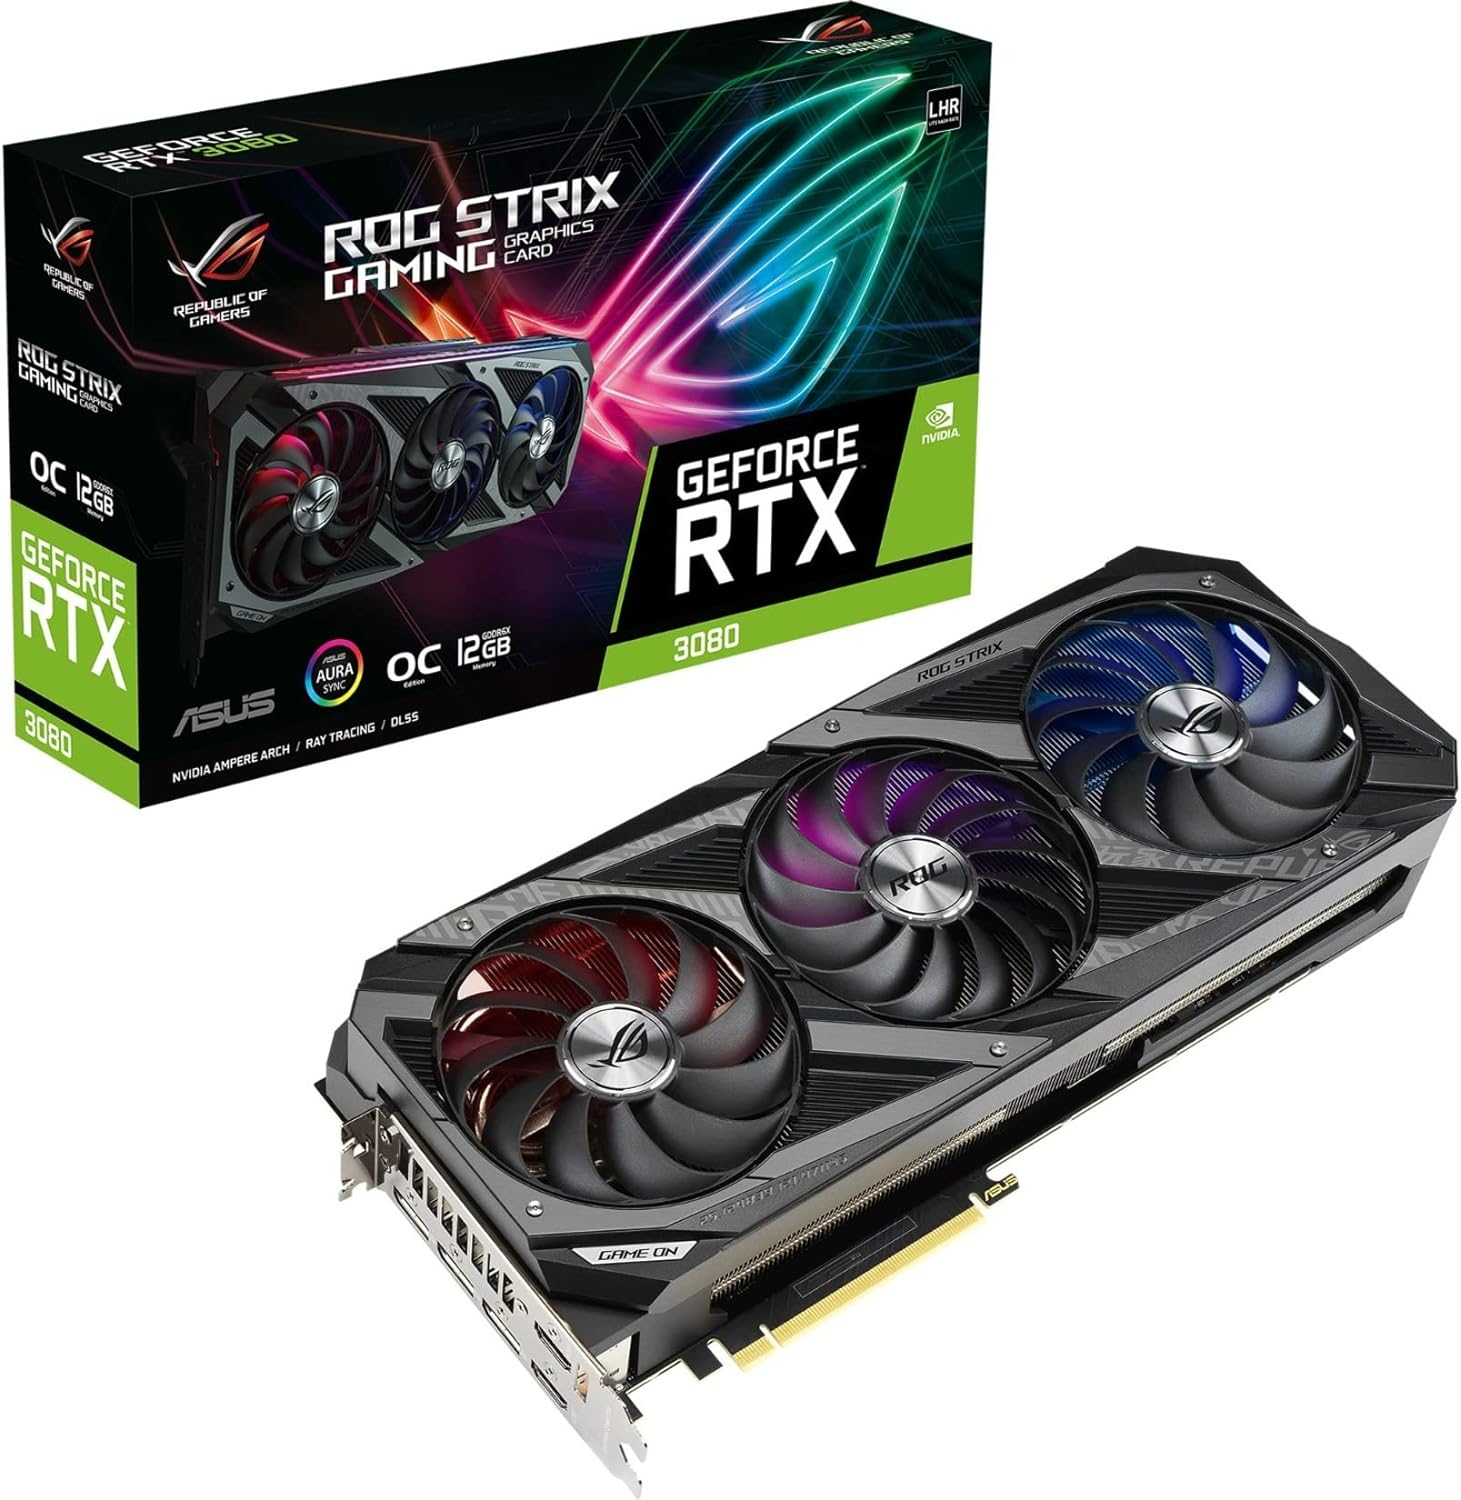
\includegraphics[width=8cm]{slike/graficka.jpg}
\caption{Asus ROG STRIX GAMING OC GeForce RTX 3080}
\end{figure}

\chapter{RAM}
Corsair Vengeance RGB Pro 32 GB (Dual Channel) DDR4, 3600 MHz
\\ RAM je odabran zbog brzine i kapaciteta. 32 GB iz razloga što često imam jako puno otvorenih programa i kartica u browseru, a 3600 MHz uvijek dobro dođe kod video obrade.
\\Cijena: 84,99€
\\Izvor:  \url{https://www.amazon.com/dp/B08SQRF8MJ?tag=pcpapi-20&linkCode=ogi&th=1&psc=1}
\begin{figure}[h]
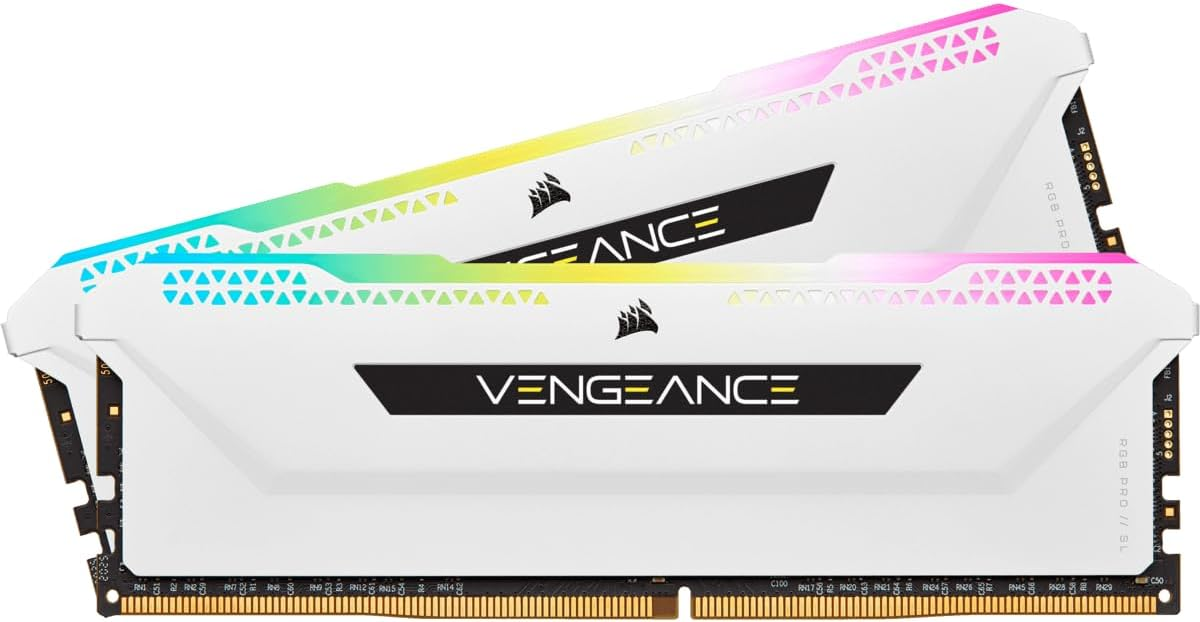
\includegraphics[width=8cm]{slike/ram.jpg}
\caption{Corsair Vengeance RGB Pro}
\end{figure}

\chapter{Matična ploča}
Asus ROG STRIX B450-F GAMING II, ATX, AM4
\\ Razlog odabira ove matične ploče je odličan design termalnih dijelova jer će mi procesor jako često biti pod opterećenjem, a i sama matična ploča je jako lijepa.
\\Cijena: 288,00€
\\Izvor:  \url{https://www.amazon.com/dp/B08KH1M1H4?tag=pcpapi-20&linkCode=ogi&th=1&psc=1}
\begin{figure}[h]
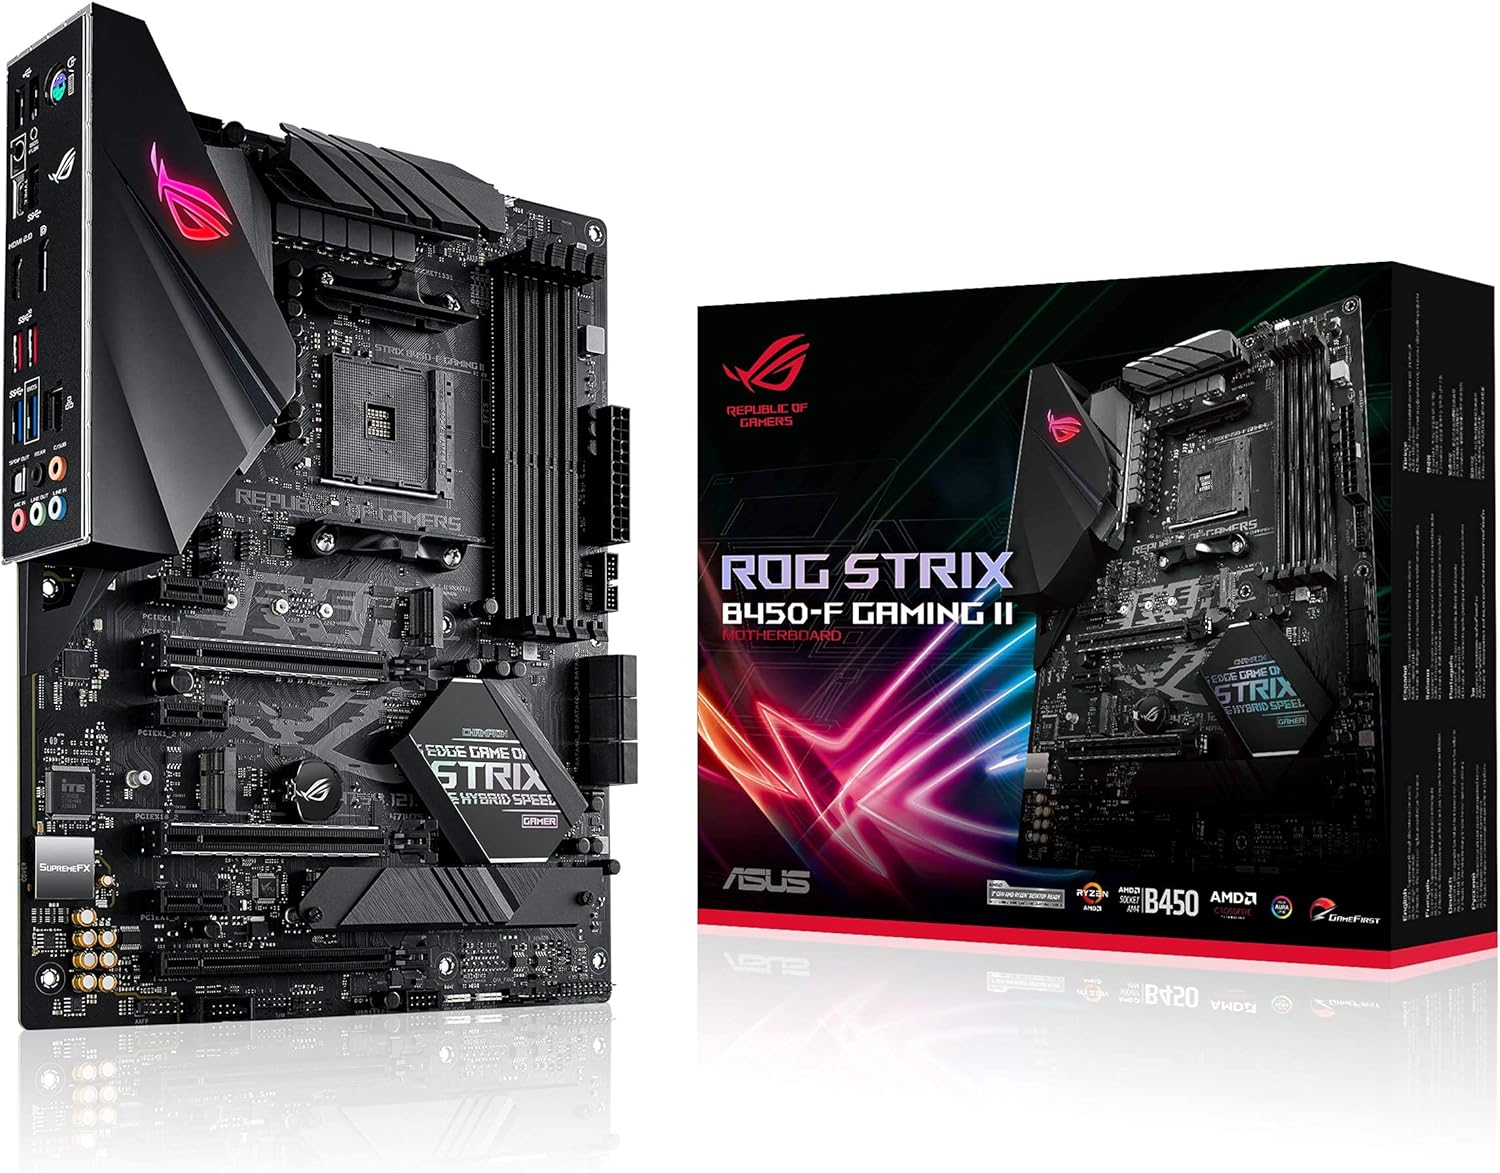
\includegraphics[width=8cm]{slike/maticna.jpg}
\caption{Asus ROG STRIX B450-F}
\end{figure}

\chapter{SSD}
Samsung 990 Pro 4 TB M.2 NVMe
\\ Ekstremno brz i dovoljno velik SSD za svakodnevnu uporabu i sva moja zanimanja. Pored ovog planiram također napraviti mali kućni server na koji mogu pohraniti sve video i foto materijale koji su često u velikim rezolucijama, što ih isto tako čini teškima.
\\Cijena: 309,99€
\\Izvor:  \url{https://www.adorama.com/ssv9p4t0bam.html?sterm=0%3AMVDsTPbxyPTlBzyXVntxOBUkHzrzxNjUX90k0&utm_source=rflaid912925&utm_medium=affiliate}
\begin{figure}[h]
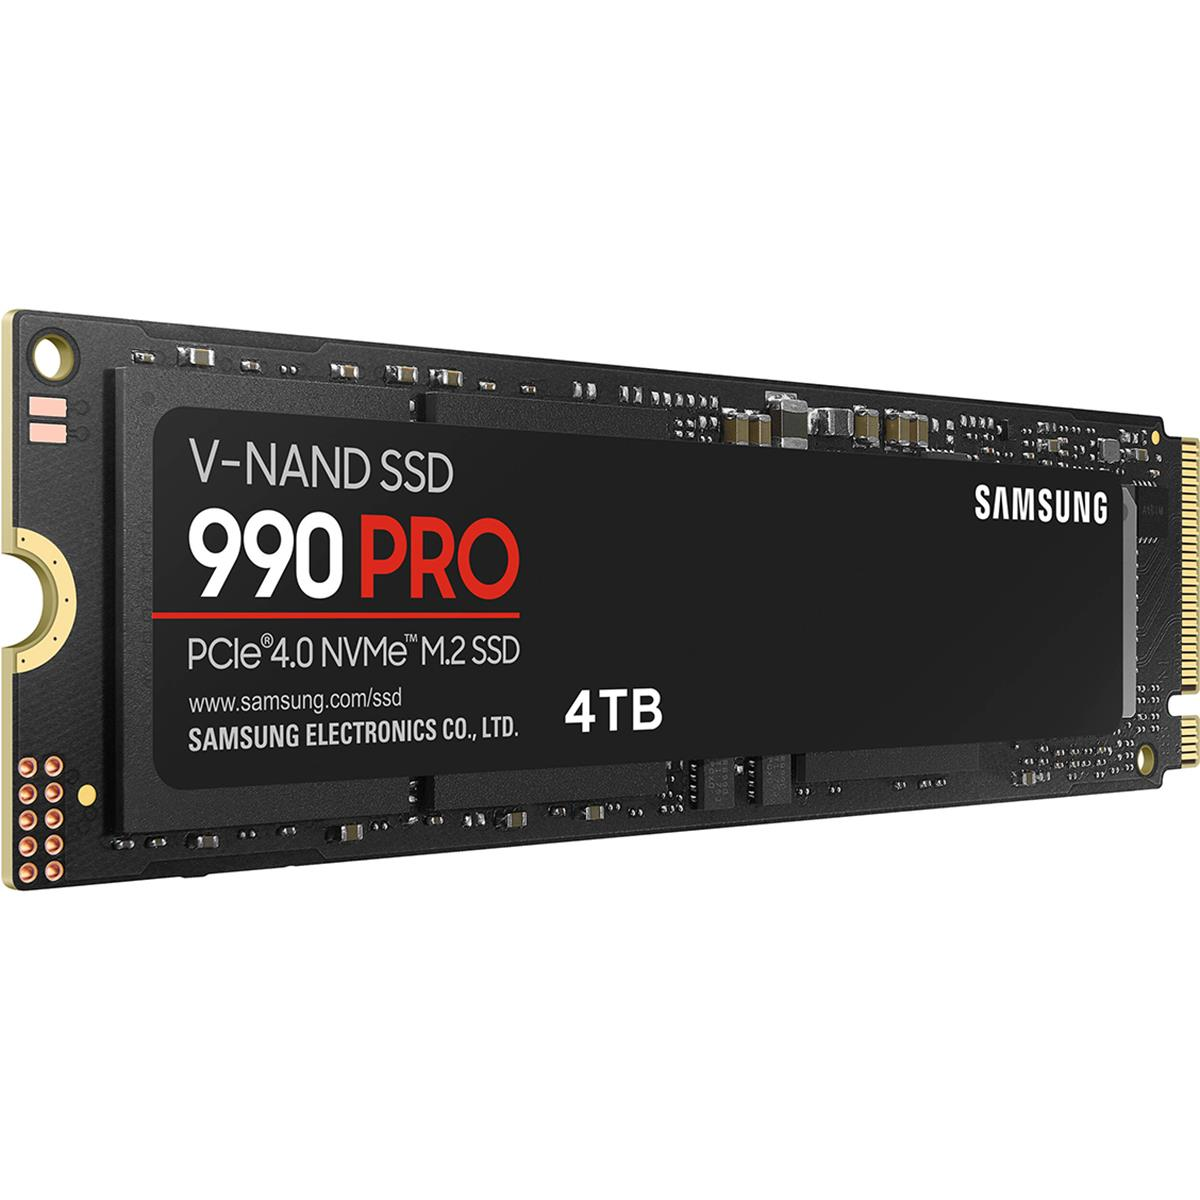
\includegraphics[width=8cm]{slike/ssd.jpg}
\caption{Samsung 990 Pro}
\end{figure}

\chapter{Hlađenje}
NZXT Kraken Elite 280 Vodeno hlađenje
\\ Odabrala sam ovo hlađenje zbog njegove veličine i recenzija. Također, ima RGB osvjetljenje koje će se lijepo uklopiti u cijeli setup.
\\Cijena: 258,70€
\\Izvor:  \url{https://www.amazon.com/dp/B0BY3GMN2V?tag=pcpapi-20&linkCode=ogi&th=1&psc=1}
\begin{figure}[h]
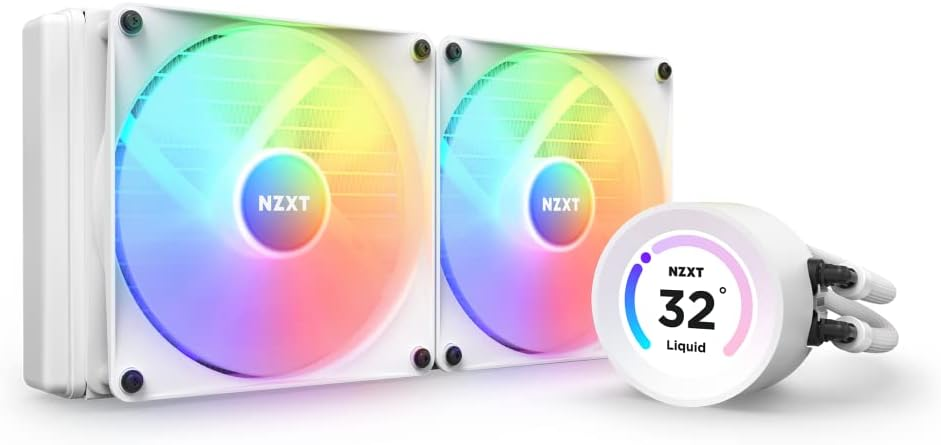
\includegraphics[width=8cm]{slike/hladnjak.jpg}
\caption{NZXT Kraken Elite 280}
\end{figure}

\chapter{Napajanje}
Asus ROG Strix 850 W 80+ Gold modularno napajanje
\\ S obzirom da mi je jako bitan izgled i estetika računala, odabrala sam ga jer je industrijski standard i zbog modularnosti. Da bi izgledalo što urednije kako bi se vidjele komponente i osvjetljenje, važno je da se nekorišteni kablovi mogu maknuti.
\\Cijena: 169,62€
\\Izvor:  \url{https://www.amazon.com/dp/B08BX7JXC3?tag=pcpapi-20&linkCode=ogi&th=1&psc=1}
\begin{figure}[h]
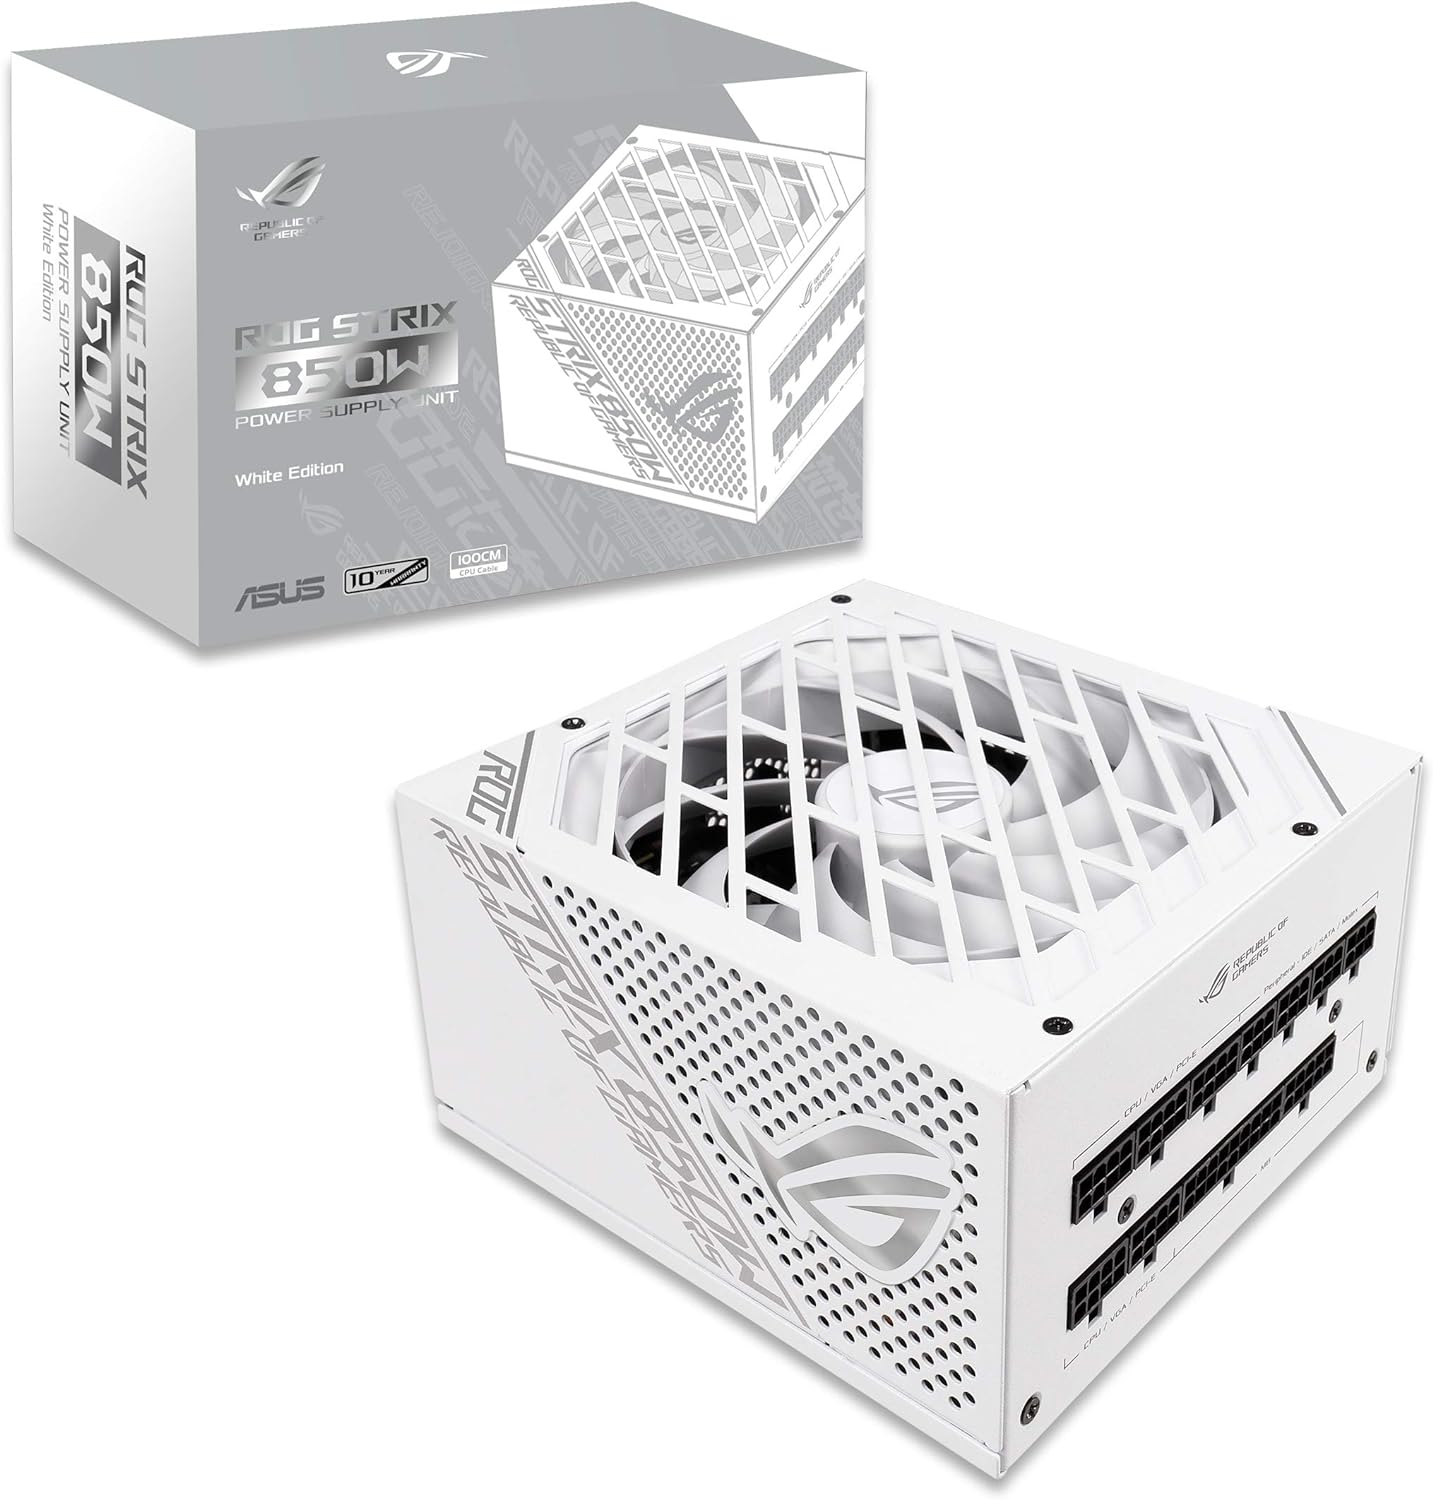
\includegraphics[width=8cm]{napajanje.jpg}
\caption{Asus ROG Strix}
\end{figure}

\chapter{Kućište}
NZXT H5 Flow ATX
\\ Da bi postigla odlične performanse, važno je imati dobar protok zraka. Također, dovoljno je veliko da se montiraju sve komponente i da podržava veliki radijator od vodenog hlađenja.
\\Cijena: 87,99€
\\Izvor:  \url{https://www.amazon.com/dp/B0B6YHDB2Y?tag=pcpapi-20&linkCode=ogi&th=1&psc=1}
\begin{figure}[h]
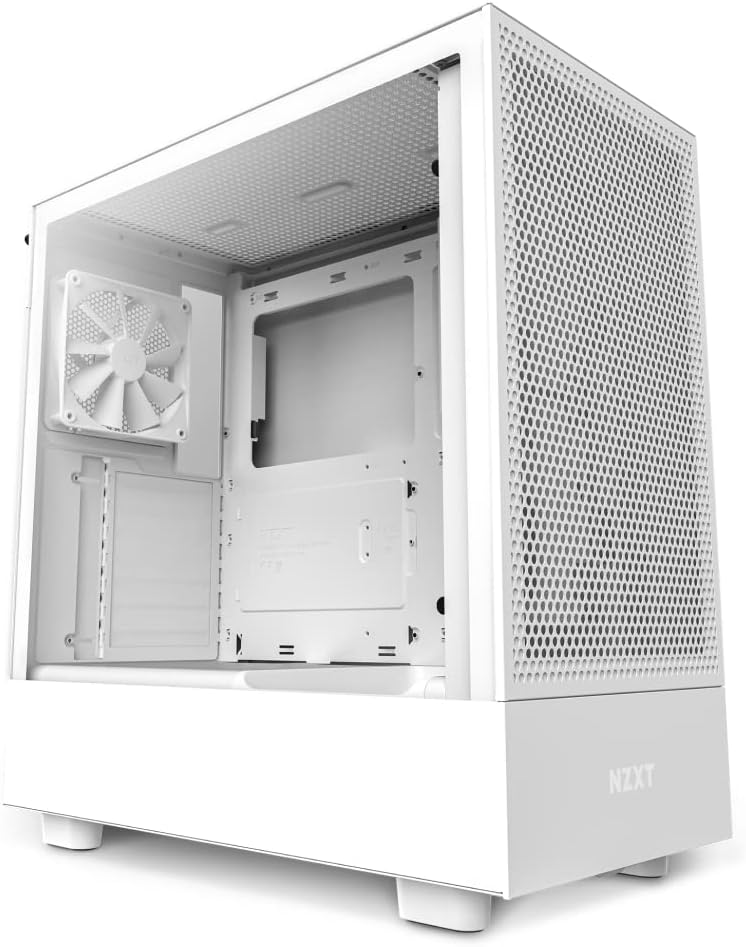
\includegraphics[height=8cm]{kuciste.jpg}
\caption{NZXT H5 Flow}
\end{figure}

\chapter{Monitor}
AOC C27G2Z 27.0" 1920 x 1080 240 Hz Curved Monitor
\\Odabrala sam ovaj monitor zbog njgove brzine osvježavanja od čak 240Hz, što je odlično za gaming. Zaobljeni oblik monitora imitira prirodan oblik oka što olakšava praćenje.
\\Cijena: 172,99€
\\Izvor:  \url{https://www.amazon.com/dp/B088LG2BSW?tag=pcpapi-20&linkCode=ogi&th=1&psc=1}
\begin{figure}[h]
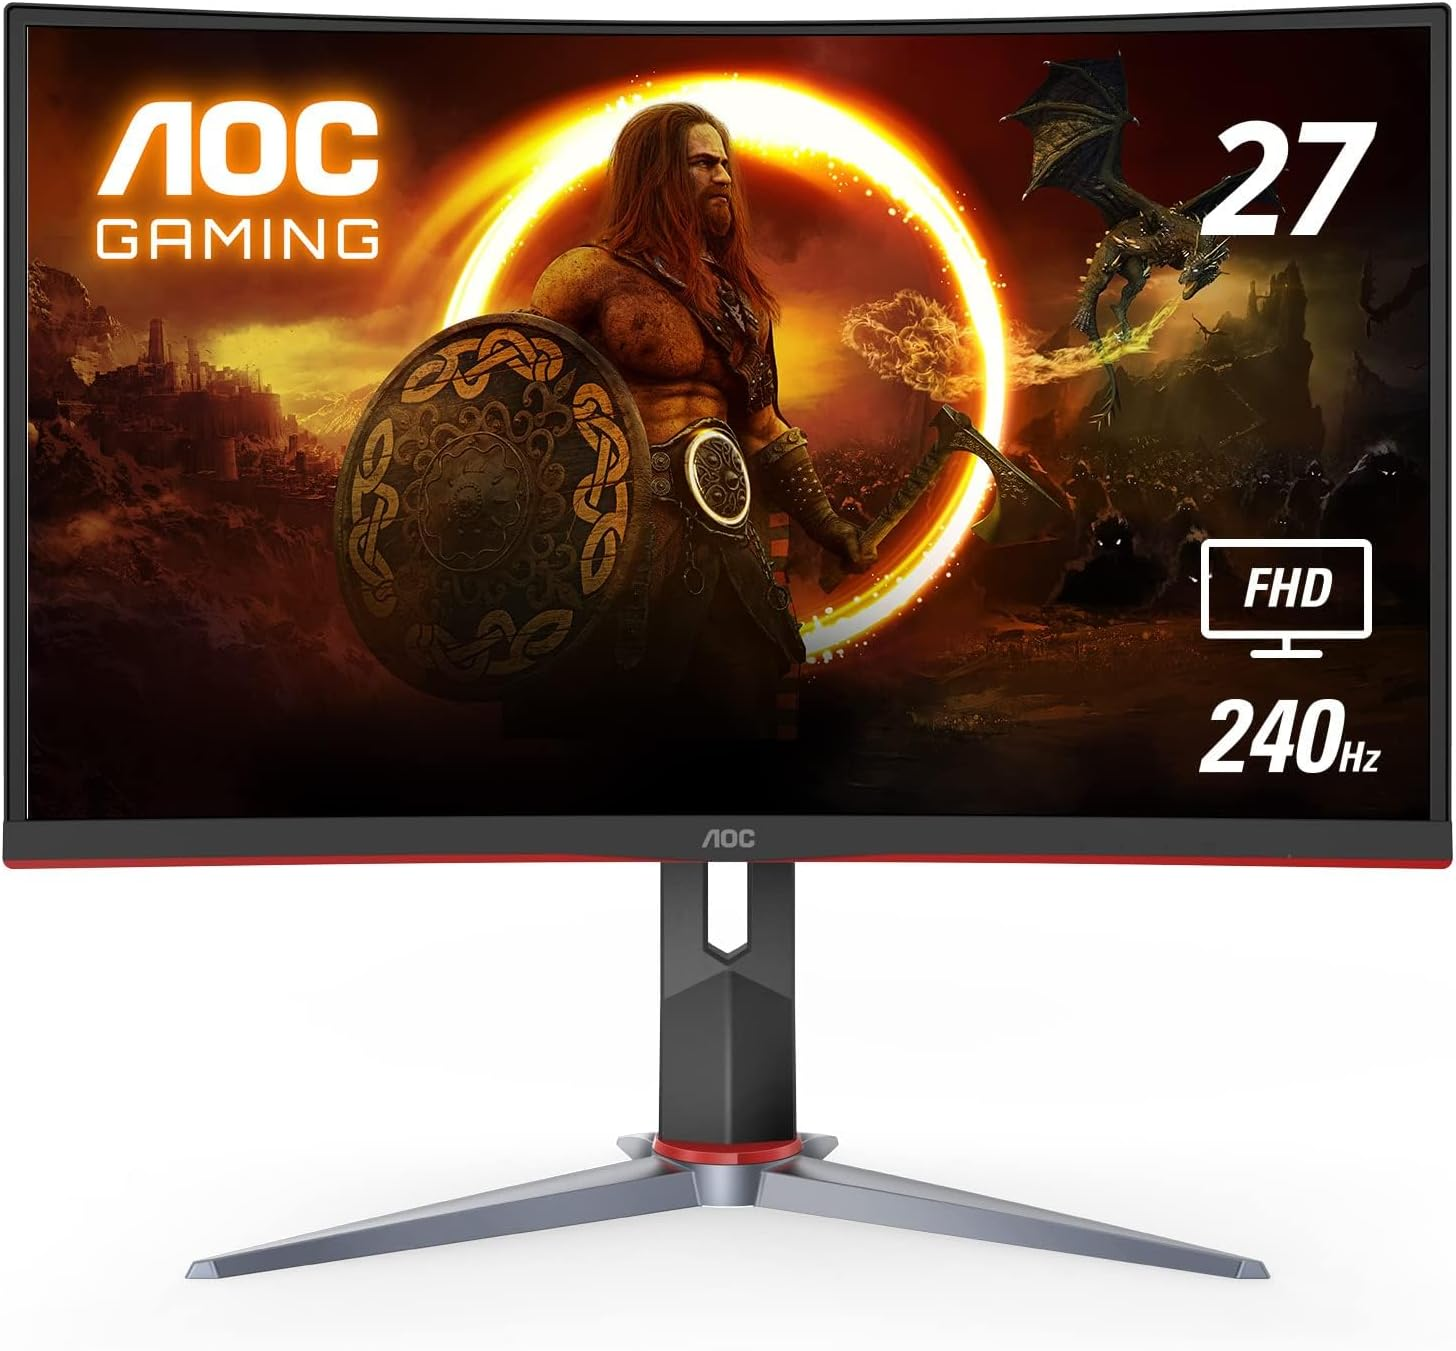
\includegraphics[width=8cm]{monitor.jpg}
\caption{AOC C27G2Z}
\end{figure}

\chapter{Tipkovnica}
Razer Pro Type Ultra Keyboard
\\Ova mehanička tipkovnica ima žute switcheve i potpuno prilagodljiv izgled preko Razer synapse 3 software-a. Veličina tipkovnice je odlična za stolno računalo,a žuti switchevi pružaju tih i mekan zvuk. Tipkovnica dolazi uz naslon za zglob koji pruža ergonomsku podršku i dodatan užitak pri korištenju.
\\Cijena: 159,99€
\\Izvor:  \url{https://www.amazon.com/Razer-Ultra-Wireless-Mechanical-Keyboard/dp/B09J72K6SM?th=1}
\begin{figure}[h]
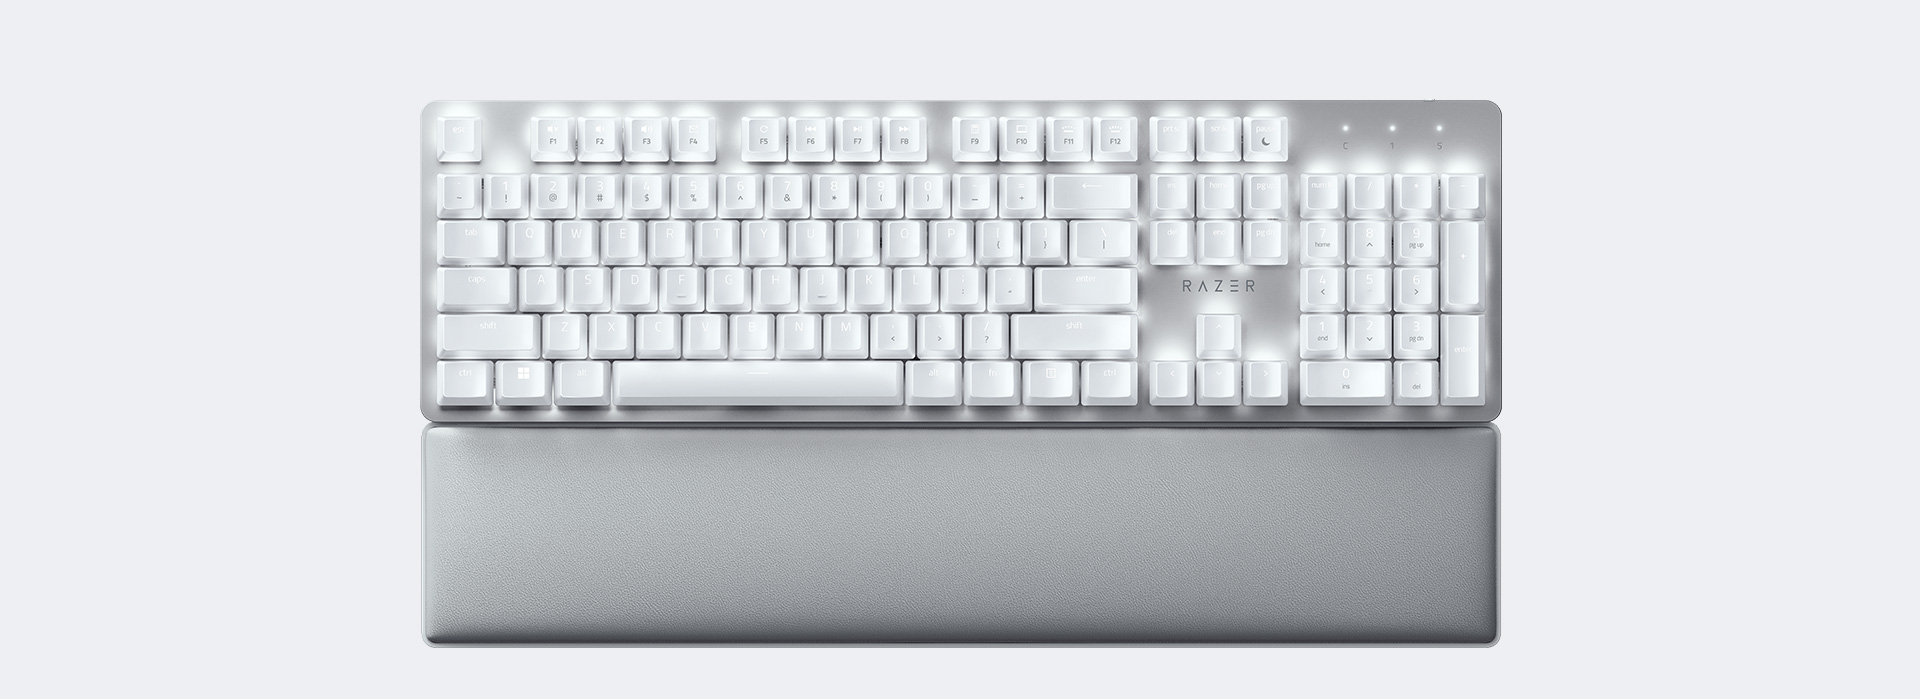
\includegraphics[width=10cm]{tipkovnica.jpg}
\caption{Razer Pro Type Ultra}
\end{figure}

\chapter{Miš}
Razer Viper V2 Pro
\\Razer Viper V2 Pro ima raspon do čak 30K DPI-a i mnogo mogućnosti za prilagođavanje. Miš je bežičan što omogućuje bolju preciznost i pokretljivost, a baterija u prosijeku traje 70 sati.
\\Cijena: 121,34€
\\Izvor:  \url{https://www.amazon.com/dp/B09VCSKB1C?tag=pcpapi-20&linkCode=ogi&th=1&psc=1}
\begin{figure}[h]
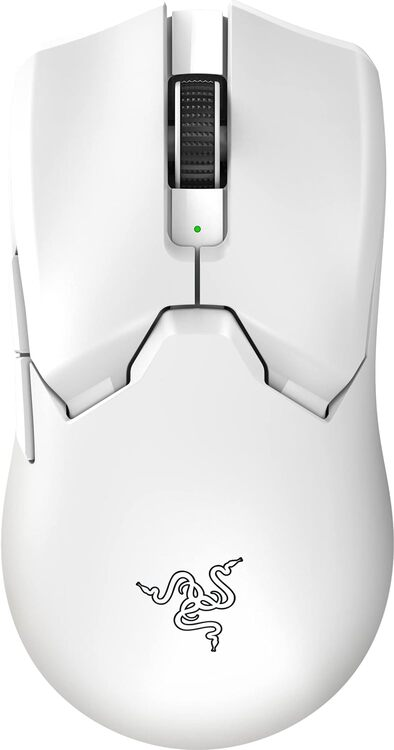
\includegraphics[height=8cm]{mis.jpg}
\caption{Razer Viper V2 Pro}
\end{figure}

\chapter{Slušalice}
Razer Kraken 7.1 V2 Mercury Edition
\\Odabrala sam ove slušalice prvenstveno zbog 7.1 surround sounda i kvalitete mikrofona. Osim što je kvaliteta zvuka odlična, slušalice se ističu i po izolaciji zvuka.
\\Cijena: 99,00€
\\Izvor:  \url{https://www.goldonecomputer.com/index.php?route=product/product&product_id=313}
\begin{figure}[h]
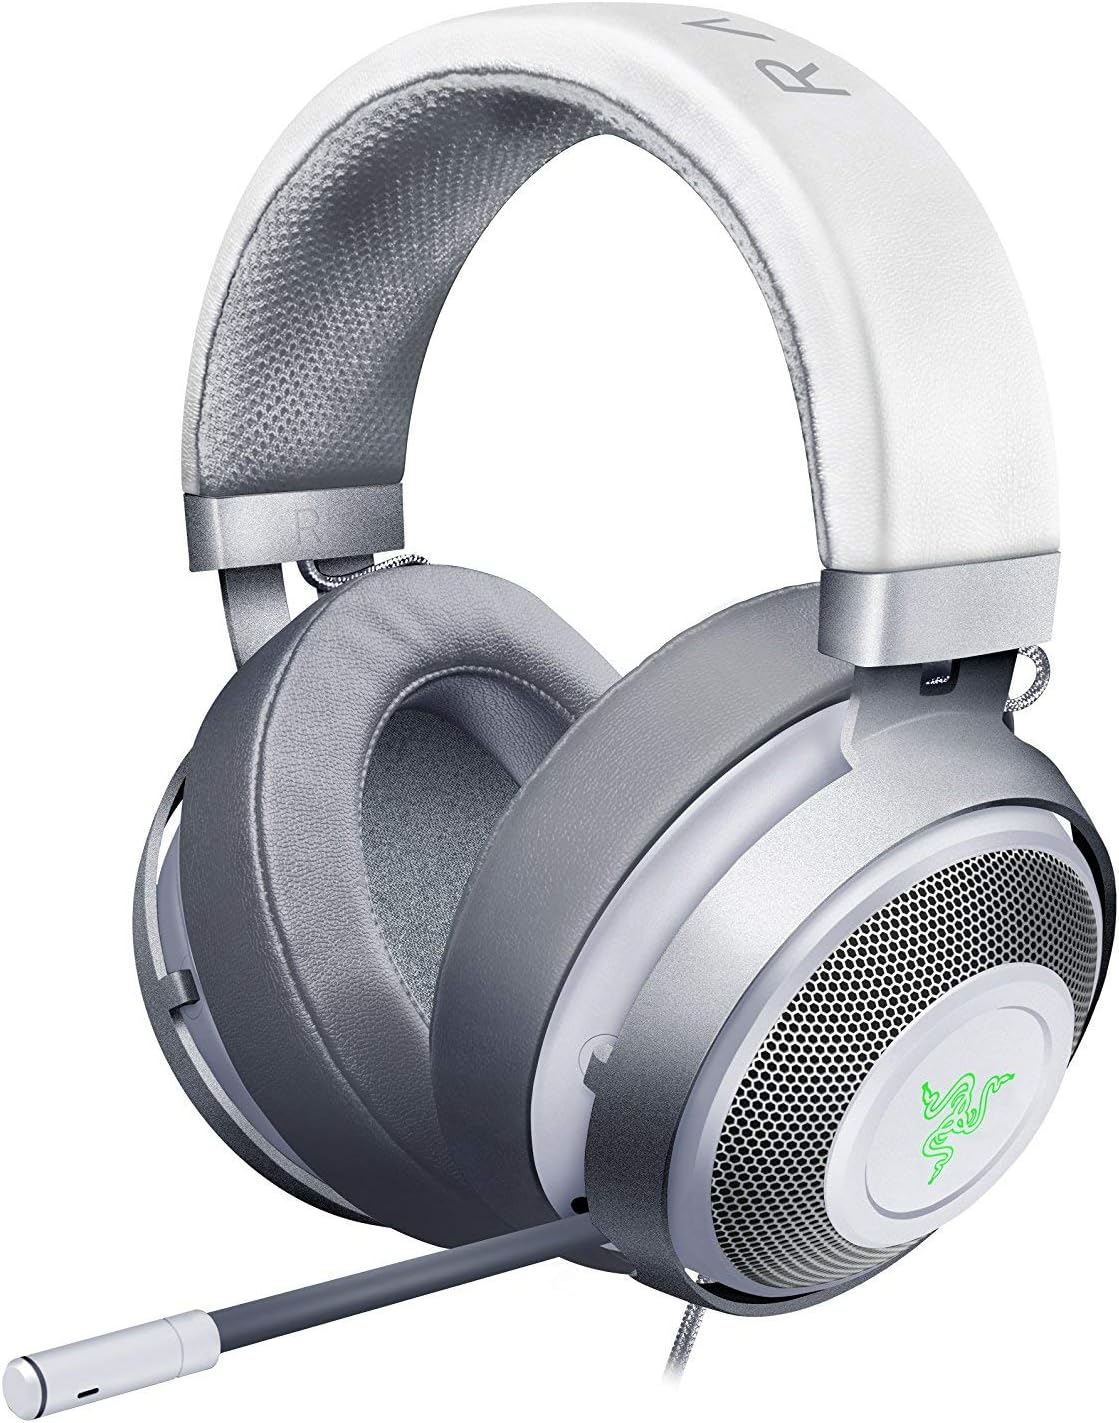
\includegraphics[height=8cm]{slusalice.jpg}
\caption{Razer Kraken V2}
\end{figure}

\end{document}